\section{Theorie}
\label{sec:theorie}

    Die Wärmekapazität eines Festkörpers bezeichnet die Wärmemenge $\symup{\Delta} Q$,
    die benötigt wird um die Temperatur $T$ dieses Festkörpers um \SI{1}{\kelvin} zu erhöhen.
    Es gilt
    \begin{equation*}
        C = \frac{\symup{\Delta}Q}{\symup{\Delta}T} \ .
    \end{equation*}
    Die Wärmekapazität ist dabei material-spezifisch und wird deshalb oft in Bezug auf eine Stoffmenge,
    ein Volumen oder eine Masse angegeben.
    Dies wird als \textit{Spezifische Wärmekapazität} bezeichnet.
    Diese ergibt sich nach \cite{grossmarx} entsprechend zu
    \begin{align*}
        c^\text{mol} = \frac{C}{\si{\mol}} && c^\text{V} = \frac{C}{V} && c^\text{mass} = \frac{C}{m} \ .
    \end{align*}
    Mithilfe des ersten Hautptsatzes der Thermodynamik
    \begin{equation}
        \symup{d}Q = \symup{d}U - \symup{d}W = \symup{d}U + p\symup{d}V
        \label{eqn:theorie:hauptsatz}
    \end{equation}
    kann zwischen der Wärmekapazität bei konstantem Volumen $C_V$ und konstantem Druck $C_p$ unterschieden werden.
    Hierbei gilt
    \begin{align*}
        C_V &= \frac{\partial Q}{\partial T} \Bigl|_V = \frac{\partial U}{\partial T} \Bigl|_V
        %\label{eqn:theorie:c_vconst}
        \\
        C_p &= \frac{\partial Q}{\partial T} \Bigl|_p = \frac{\partial U}{\partial T} \Bigl|_p \ .
        %\label{eqn:theorie:c_pconst}
    \end{align*}
    Weiterhin ergibt sich die Differenz
    \begin{equation}
        C_p - C_V = T \alpha^2_V B V = 9 \alpha^2 \kappa V_0 T
        \label{eqn:theorie:c_differenz}
    \end{equation}
    mit dem Ausdehnungskoeffizenten $\alpha$,
    dem Bulkmodul $B$ und dem Kompressionsmodul $\kappa$.
    Diese Differenz ist im Allgemeinen $\geq 0$,
    da $C_p \geq C_V$ ist,
    was daran liegt,
    dass nach \autoref{eqn:theorie:hauptsatz} bei konstantem Druck mehr Energie auf die Ausdehnung des Volumens aufgewendet werden muss,
    sodass mehr Wärme benötigt wird,
    um die gleiche Temperatur zu erreichen.
    Aus diesem Grund ist die Differenz \autoref{eqn:theorie:c_differenz} im Falle eines Festkörpers geringer als bei einem idealen Gas,
    da sich der Festkörper weniger stark ausdehnt,
    wenn er erwärmt wird.

    Im Folgenden wird zwischen \textit{klassischer} und \textit{quantenmechanischer} Betrachtung unterschieden.
    Zusätzlich werden die Schwingungsmoden im Festkörper als harmonische Oszillatoren behandelt.

    In der klassischen Betrachtung kann ein System,
    welches in Kontakt mit einem Wärmebad ist,
    bei jeder Temperatur angeregt werden,
    da der klassische harmonische Oszillator ein kontinuierliches Energiespektrum besitzt.
    Jede Schwingungsmode hat dabei eine mittlere Energie von $\sfrac{1}{2} k_\text{B} T$.
    Ein dreidimensionales System mit $N$ Atomen,
    drei Ortsfreiheitsgraden und drei Impulsfreiheitsgraden hat demnach eine Energie von $3Nk_\text{B}T$ und demnach eine Wärmekapazität von $3Nk_\text{B}$.
    Dieser Zusammenhang wird als \textit{Dulong-Petit-Gesetz} bezeichnet und stellt den Hochtemperaturgrenzfall der Wärmekapazität dar.

    In der quantenmechanischen Betrachtung muss die Bedingung $\hbar \omega \ll k_\text{B} T$ erfüllt sein.
    Der Grund dafür besteht darin,
    dass der quantenmechanische harmonische Oszillator nur diskrete Energiewerte $\hbar \omega (n+\sfrac{1}{2})$ besitzt.
    Die zugeführte Energie durch das Wärmebad muss dementsprechend größer als die Energiedifferenz sein,
    damit der Oszillator angeregt werden kann.
    Wenn die Temperatur kleiner ist,
    werden keine Moden mehr angeregt.
    Dies wird auch als \textit{Ausfrieren der Moden} bezeichnet.

    Im Folgenden sollen das \textit{Einstein}- und das \textit{Debye-Modell} vorgestellt werden,
    welche eine Näherung der Wärmekapazität für hohe und tiefe Temperaturen geben.
    Dabei wird vor allem auf die unterschiedliche Betrachtung der Moden im Festkörper eingegangen.
    Im Allgemeinen besitzt jeder Festkörper drei \textit{optische} Moden und $3R-3$ \textit{akustische} Moden.
    Die Moden können auch über Quasiteilchen,
    sogenannte \textit{Phononen},
    beschrieben werden,
    welche die Gitterschwingungen darstellen.
    Die entsprechende Dispersionsrelation ist in \autoref{fig:theorie:moden} dargestellt.
    \begin{figure}
        \centering
        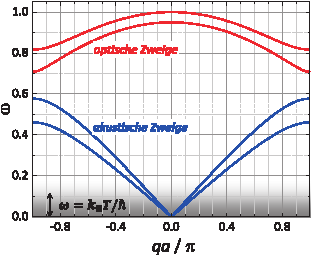
\includegraphics[width=0.5\textwidth]{content/img/Gross_Marx/6_4.pdf}
        \caption{Darstellung der Dispersionsrelation in einem Festkörper. Es wird zwischen optischen und akustischen Moden unterschieden. \cite{grossmarx}}
        \label{fig:theorie:moden}
    \end{figure}

\subsection{Das Einstein-Modell}
\label{sec:theorie:einstein}

    Das Einstein-Modell betrachtet $3N$ Eigenschwingungen mit der gleichen Frequenz $\omega_\text{E}$.
    In \autoref{fig:theorie:moden} würde dies einer Konstanten entsprechen,
    die auf Höhe der optischen Mode eingezeichnet würde.
    Es ergibt sich eine Einstein-Temperatur $\Theta_\text{E} = \sfrac{\hbar \omega_\text{E}}{k_\text{B}}$.
    Für die Wärmekapazität gilt damit
    \begin{equation*}
        C^{\text{E}}_V =
        \begin{cases}
            3Nk_\text{B} \Bigl(\frac{\Theta_\text{E}}{T}\Bigr)^2 \exp\Bigl(\frac{-\Theta_\text{E}}{T}\Bigr) & , T \ll \Theta_\text{E} \\
            3Nk_\text{B} & , T \gg \Theta_\text{E} \ .
        \end{cases}
    \end{equation*}

    Bei hohen Temperaturen erfüllt das Einstein-Modell die Erwartung von Dulong-Petit,
    allerdings ergibt sich bei tiefen Temperaturen nicht die beobachtete $T^3$-Abhängigkeit.
    Dies liegt daran,
    dass in diesem Modell nur die optischen Moden betrachtet werden,
    welche den Verlauf der Wärmekapazität für tiefe Temperaturen nicht gut beschreiben.

\subsection{Das Debye-Modell}
\label{sec:theorie:debye}

    Im Debye-Modell werden nun alle Moden durch drei Moden mit einer linearen Dispersionsrelation $\omega = v_i q$ angenähert.
    Mithilfe des Debye-Wellenvektors $q_\text{D}$ und der Zustandsdichte
    \begin{equation*}
        D(\omega) = \frac{V}{2 \pi^2}{\omega^3}{v^3_i}
    \end{equation*}
    ergibt sich die Debye-Frequenz
    \begin{equation*}
        \omega_\text{D} = v_i \Bigl(6 \pi^2 \frac{N}{V}\Bigr)^{\frac{1}{3}} \ ,
    \end{equation*}
    über das Intergral
    \begin{equation*}
        \int_0^{\omega_\text{D}} D(\omega) \symup{d}\omega = 3N \ .
    \end{equation*}
    Die Schallgeschwindigkeit der jeweiligen Mode ist über $v_i$ gegeben.
    Die gesamte Schallgeschwindigkeit kann zu
    \begin{equation}
        \frac{1}{v^3_\text{s}} = \frac{1}{3} \sum_{i=1}^3 \frac{1}{v^3_i}
        \label{eqn:theorie:schallgeschwindigkeit}
    \end{equation}
    berechnet werden.

    Die zugehörige Debye-Temperatur gilt $\Theta_\text{D} = \sfrac{\hbar\omega_\text{D}}{k_\text{B}}$.
    Für die Wärmekapazität folgt
    \begin{equation*}
        C^\text{D}_V = 9Nk_\text{B} \Bigl(\frac{T}{\Theta_\text{D}}\Bigr) ^3
        \int_0^{\sfrac{\Theta_\text{D}}{T}} \frac{x^4 \symup{e}^x}{(\symup{e}^x - 1)^2} \symup{d}x =
        \begin{cases}
            \frac{12}{5} \pi^2 N k_\text{B} \Bigl(\frac{T}{\Theta_\text{D}}\Bigr)^3 & , T \ll \Theta_\text{D} \\
            3Nk_\text{B} & , T \gg \Theta_\text{D} \ .
        \end{cases}
    \end{equation*}
    Für die Hochtemperaturnäherung ergibt sich wieder Dulong-Petit und für die Tieftemperaturnäherung die erwartete $T^3$-Abhängigkeit.
    Die Debye-Temperatur kann auch als Übergang zwischen klassischer und quantenmechanischer Betrachtung angesehen werden.
    Im Fall $T > \Theta_\text{D}$ ergibt sich der klassische Fall,
    da alle Moden angeregt werden können.
    Für $T < \Theta_\text{D}$ gilt der quantenmechanische Fall,
    es befinden sich mehr – oder alle – Oszillatoren im Grundzustand und die Moden frieren aus.

    Die \autoref{fig:theorie:modelle} zeigt den Verlauf der Wärmekapazität im Einstein- und im Debye-Modell.
    \begin{figure}
        \centering
        \begin{subfigure}{0.48\textwidth}
            \centering
            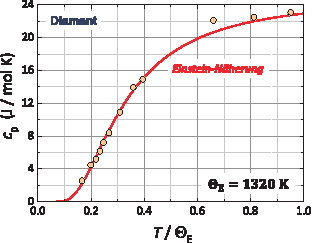
\includegraphics[width=1\textwidth]{content/img/Gross_Marx/6_5.pdf}
            \caption{Wärmekapazität im Einstein-Modell.}
            \label{fig:theorie:einsteinmodell}
        \end{subfigure}
        \hfill
        \begin{subfigure}{0.48\textwidth}
            \centering
            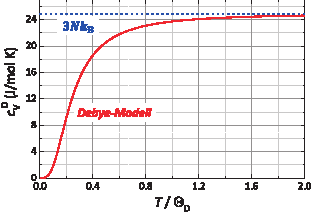
\includegraphics[width=1\textwidth]{content/img/Gross_Marx/6_7.pdf}
            \caption{Wärmekapazität im Debye-Modell.}
            \label{fig:theorie:debyemodell}
        \end{subfigure}
        \caption{Verlauf der Wärmekapazität im Einstein- und im Debye-Modell.
        In beiden Fällen nähert sich der Wert für hohe Temperaturen dem klassischen Grenzfall von Dulong-Petit an. \cite{grossmarx}}
        \label{fig:theorie:modelle}
    \end{figure}

